\chapter{Experiments and Lab Work}\label{ch:experiment}
To relate the theory behind controlling pumps to the real world,
we conducted different experiments.
This helped to gain knowledge about the pump system,
to test controller implementations, and to gather the data needed for tuning of the controller.

\section{Data Acquisition}\label{sec:data_gathering}
The pump system is built as described in Chapter \ref{ch:physsetup},
with the controlling PC running xPC Target,
a real-time OS for use with SLRT. 

All data was collected with the help of custom made 
ML scripts and SLRT models.
The execution of these was done on the xPC Target OS.
Specific parts of these files will be explained in this chapter,
while the complete files can be found on the GitHub repository \cite{GitHub}.

To use SLRT on xPC targets, a SL model of the system was made on the host PC,
compiled, transferred over Ethernet and executed on the xPC target.
After the real-time execution is finished on the target,
the .dat files containing the recorded data have to be transferred back to the host,
where further analysis can be done.

To automate as much of this process as possible,
we created a ML script that updates and compiles the SL model, transfers it to the target,
starts the execution and copies the generated .dat files to the host.

\section{System Test}\label{sec:system_test} 

\todo[color=05ExperimentsAndLabWork]{refer back to physical setup}
To obtain information about how the system reacts under different conditions,
a test was carried out with some example conditions.
From those conditions, the goal is to extrapolate an equation for the system,
that can estimate the systems reaction at different conditions.
To obtain the data needed,
a single pump is run at different speeds,
while flow resistance is varied by a choke valve,
resulting in corresponding values of flow, pressure, and energy consumption
measured by the sensors.
The measured data was stored for further analysis such as creating pump curves.

To get an overview over the whole operating range of the setup,
a very broad test was conducted.
We wanted to find the correlations between pump speed, backpressure, flow and power consumption.
To get reliable results, we chose to only change one variable at a time.
Since the value to be changed by our controller was expected to be the pump speed $\omega P_{1,2,3}$,
we decided to fix the backpressure by fixing the control valve position,
and stepwise change $\omega P_{1,2,3}$.
Since the three pumps in the setup are expected to be identical,
the test was only run with one of the pumps.
We chose to use pump 2 at random.

\subsection{Gathered Data}
Several tests were done on the setup, in order to get a general overview of the system.
Pump 2 was chosen at random.
We have run several tests, where we have gradually changed the pump speed in order to monitor
the flow, pressure and power consumption.
Starting from 0\% pump speed ($\omega P$), we have increased $\omega P$ by 10\% every 15 seconds.
This was done in order to give the system some time to stabilize.
The process was repeated for a range of valve openings.
Similar to $\omega P$, the valve was in the beginning 10\% open,
gradually increasing by 10\% and finally reaching 100\%.
Several identical tests were conducted, in order to see if the values would hold.

Figure \ref{fig:measuredFlow} shows the raw flow measurements,
while Figure \ref{fig:measuredPower} shows the raw power measurements.
Interesting to notice here is that the lowest values for $Q$ appeared at the lowest values for $CV_1$,
while $P$ behaves in the opposite manner, having its highest values at the lowest $CV_1$.
\begin{figure}[H]
	\centering
	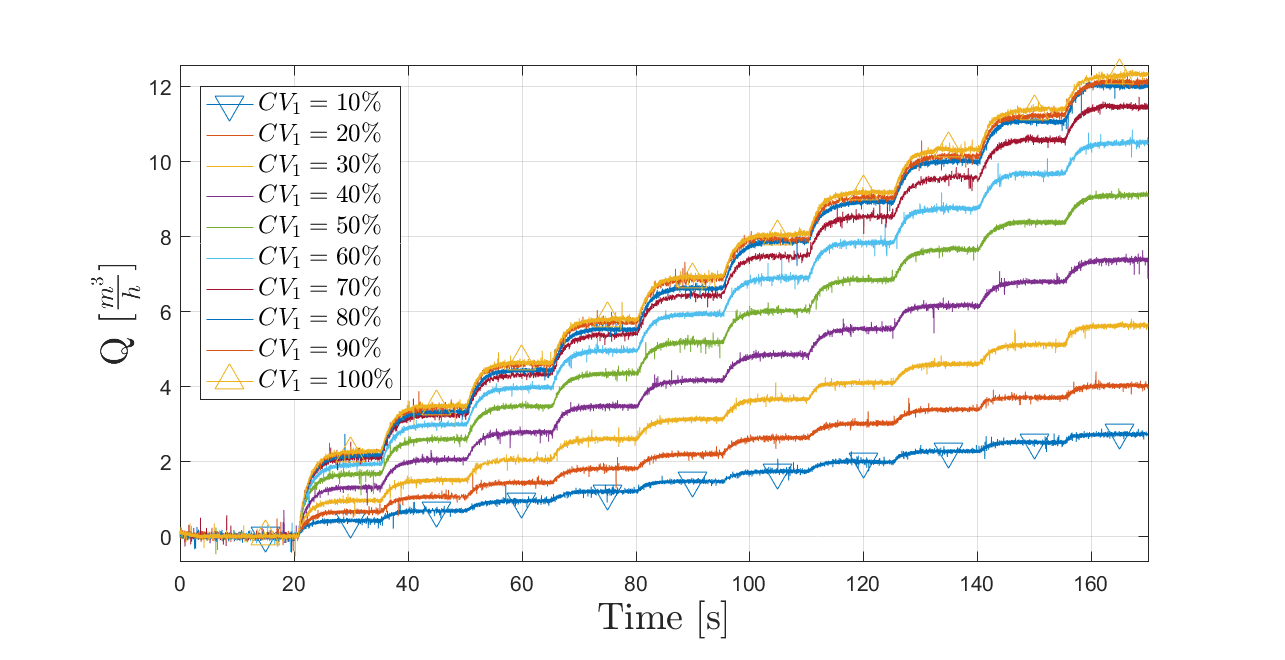
\includegraphics[width=0.8\textwidth]{figures/05mathematicalModelling/measuredFlow.eps}
	\caption{Measured Flow}
	\label{fig:measuredFlow}
\end{figure}

\begin{figure}[H]
	\centering
	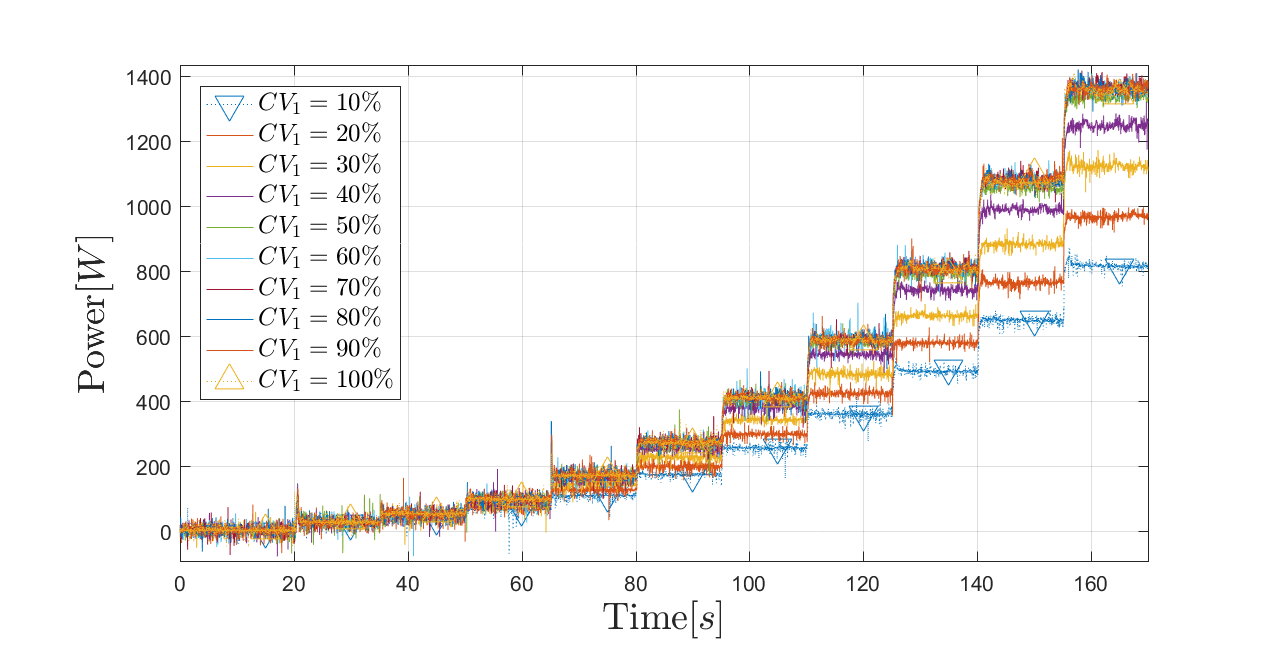
\includegraphics[width=0.8\textwidth]{figures/05mathematicalModelling/measuredPower.eps}
	\caption{Measured Power}
	\label{fig:measuredPower}
\end{figure}

\begin{figure}[H]
	\centering
	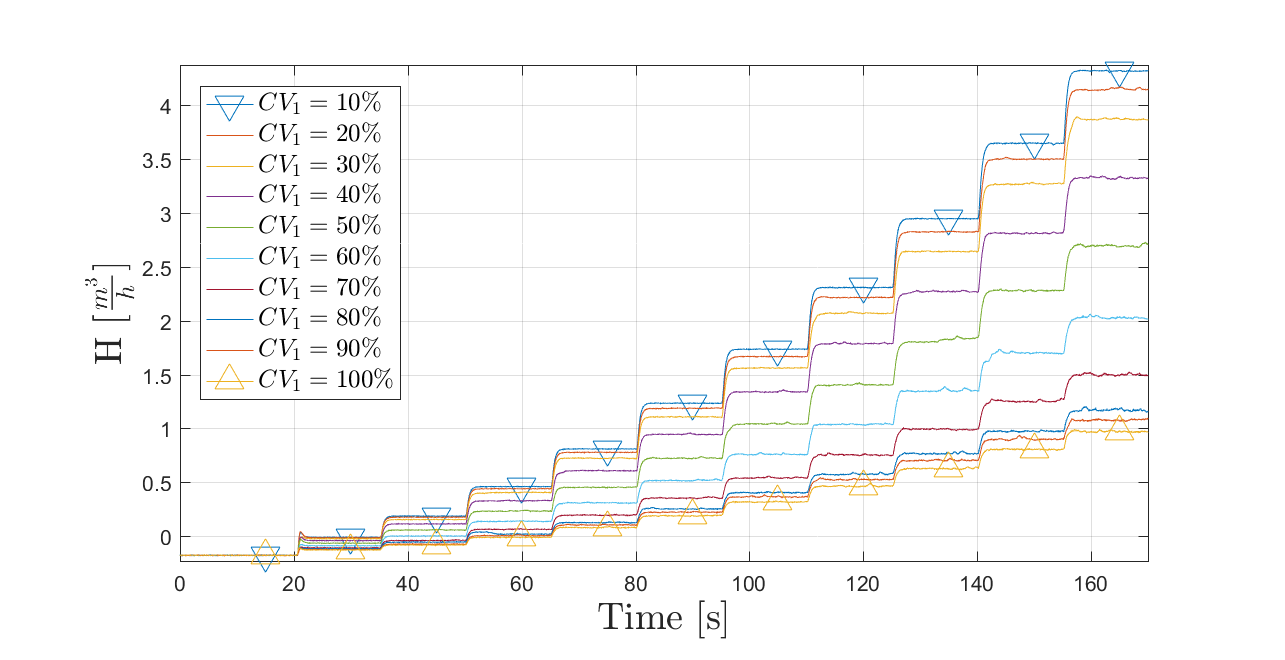
\includegraphics[width=0.8\textwidth]{figures/05mathematicalModelling/measuredPressure.eps}
	\caption{Measured Pressure}
	\label{fig:measuredPressure}
\end{figure}

\todo[color=05ExperimentsAndLabWork]{fix formatting later and also add for pressure}

\subsection{Data Example}%\label{sec:results}
To give some more insight in the testing,
we wanted to show the data collected in a single run.
The Figures \ref{fig:measuredFlow}, \ref{fig:measuredPower} and \ref{fig:measuredPressure}
show the collected data through several runs,
each with a different $CV_1$.
The data for all lines $CV_1 = 70\%$ in all three figures comes from the same run.
While executing a run,
the data for all used sensors was shown on the target in real time.
To get a better understanding of how the tests were executed,
we included Figure \ref{fig:testrun},
a rebuilt live view.

\begin{figure}[H]
	\centering
	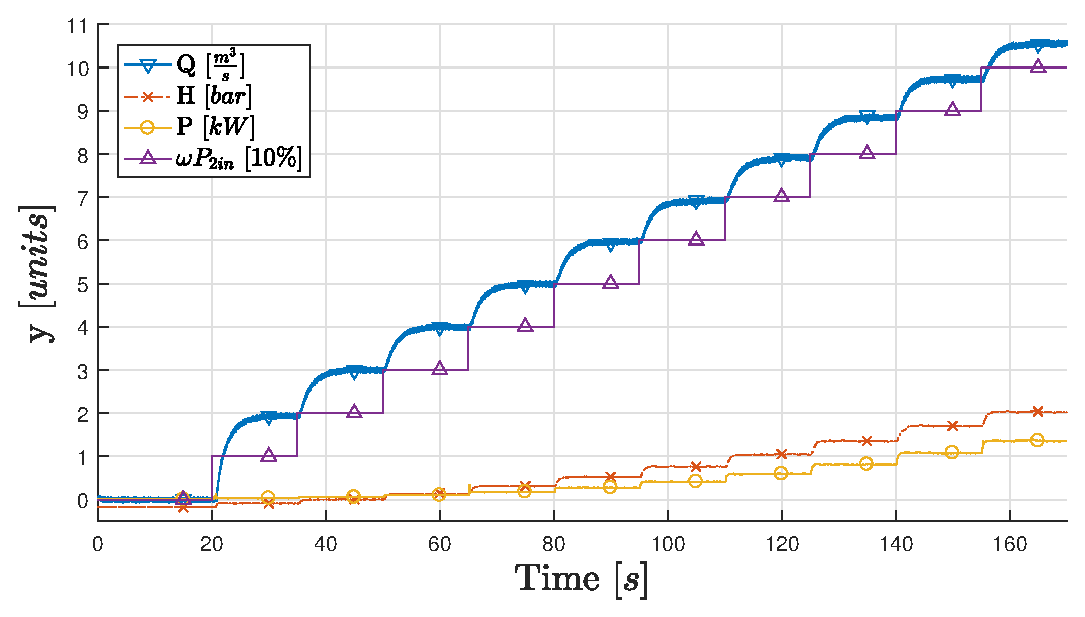
\includegraphics[width=0.8\textwidth]{figures/04ExperimentsAndLabWork/testrun.eps}
	\caption{$Q$, $H$, $P$ and stair input $\omega P_{2in}$ at $CV_1 = 70\%$}
	\label{fig:testrun}
\end{figure}
In this test $\omega P$ was stepwise increased while $CV_1$ was fixed at 70\%.
\todo[color=05ExperimentsAndLabWork]{I think this sentence can go --Daniel}
